
\subsection{問題1:3ノードの単純なネットワーク}

図~\ref{fig:quiz01}のようなネットワークがあるとする。
このとき、ノードh1からノードh3へ及び、ノードh3からノードh1へIPv4パケットが到達するように、
ノードh1〜h3を設定せよ。ただし、ブリッジ接続ではなく、
ルーティングテーブルを設定してL3レベルでの設定を行うこと。
ヒント:ノードh1〜h3のルーティングテーブルをrouteコマンドで設定し、
ノードh2をIPv4のフォワーディングを行うようにsysctlコマンドで設定せよ。

\begin{figure}
    \centering
    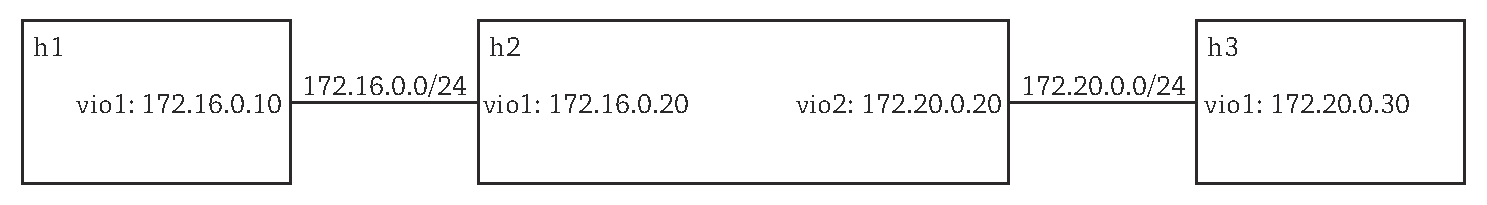
\includegraphics[width=15cm,pagebox=artbox]{figs/quiz01.pdf}
    \caption{問題1:ルーティング実験の3ノードトポロジ図} \label{fig:quiz01}
\end{figure}

\subsection{問題2:4ノードのネットワーク}

図~\ref{fig:quiz02}のようなネットワークがあるとする。
このとき、各ノードから全てのノードへIPv4パケットが到達するように、
ノードh1〜h4を設定せよ。
ただし、ブリッジ接続ではなく、
ルーティングテーブルを設定してL3レベルでの設定を行うこと。

\begin{figure}
    \centering
    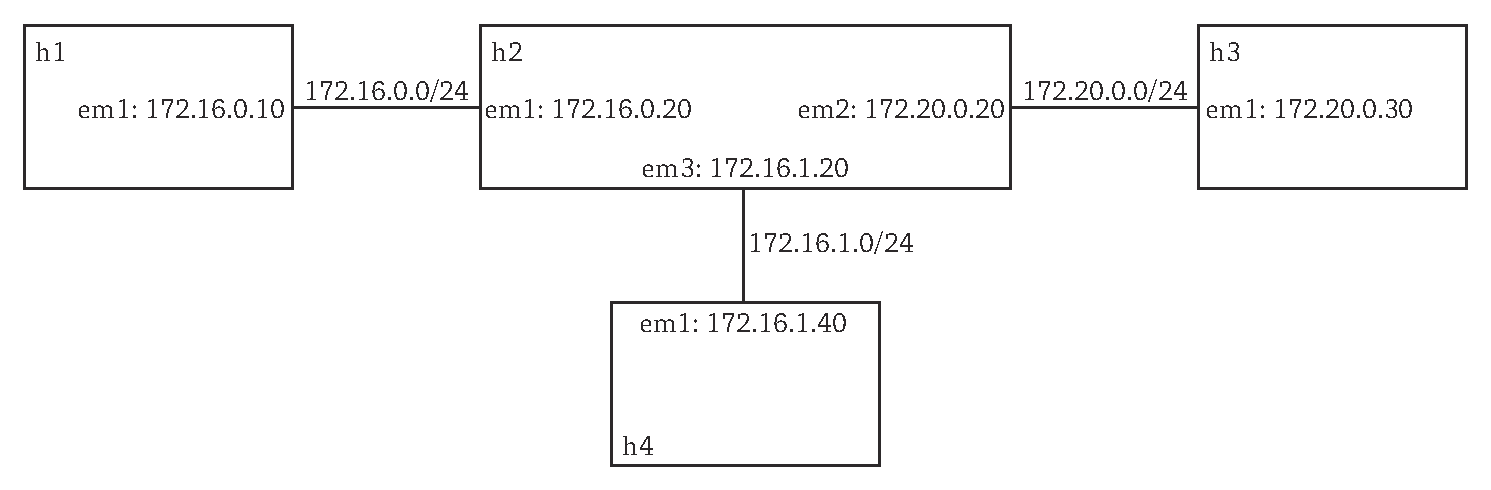
\includegraphics[width=15cm,pagebox=artbox]{figs/quiz02.pdf}
    \caption{問題2および3:ルーティング実験、DMZ実験の4ノードトポロジ図} \label{fig:quiz02}
\end{figure}

\subsection{問題3:DMZ(DeMilitarized Zone)}

同じく、図~\ref{fig:quiz02}のネットワークを利用して、以下の要求を満たすように
サービスを構築し、ノードh2にpfでファイアウォールを構築せよ。
ファイアウォールの設定後は、ping、curlコマンドなどを利用して設定が要求どおりとなっているか確認すること。

\begin{itemize}
    \item ノードh1の所属するネットワーク172.16.0.0/24を社内ネットワークとする
    \item ノードh3の所属するネットワーク172.16.20.0/24をインターネットに接続するための対外ネットワークとする
    \item ノードh4の所属するネットワーク172.16.1.0/24を対外向けサービスを設置するためのDMZネットワークとする
    \item ノードh1、h3、h4にWebサーバを構築せよ
    \item 社内ネットワークから対外ネットワーク及びDMZネットワークへのTCP、UDP、ICMP接続が可能
    \item DMZネットワークから社内ネットワークへのTCP、UDP、ICMP接続は禁止
    \item DMZネットワークから対外ネットワークへのTCP、UDP、ICMP接続は可能
    \item 対外ネットワークからDMZネットワークへの接続はWebのみ可能
    \item 対外ネットワークから社内ネットワークへのTCP、UDP、ICMP接続は禁止
\end{itemize}

\subsection{問題4:内部サービスを分離したネットワーク}

\begin{figure}
    \centering
    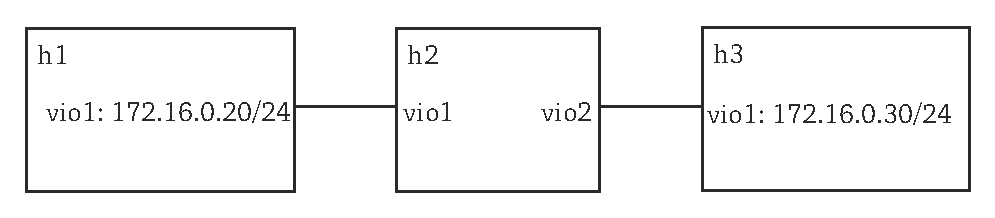
\includegraphics[width=15cm,pagebox=artbox]{figs/quiz04.pdf}
    \caption{問題4:内部サービスを分離したトポロジ図} \label{fig:quiz04}
\end{figure}

図~\ref{fig:quiz04}のネットワークのは、問題3(図~\ref{fig:quiz02})に
社内サービス用のネットワーク172.16.2.0/24、ノードh5を追加したネットワークトポロジとなっている。
社内ネットワークに対するファイアウォールの設定はどのようにすればよいだろうか?
まず、問題3のように要求を定義し、その後実際に各ノードおよびファイアウォールを設定せよ。

\subsection{問題5:ブリッジ}

\begin{figure}
    \centering
    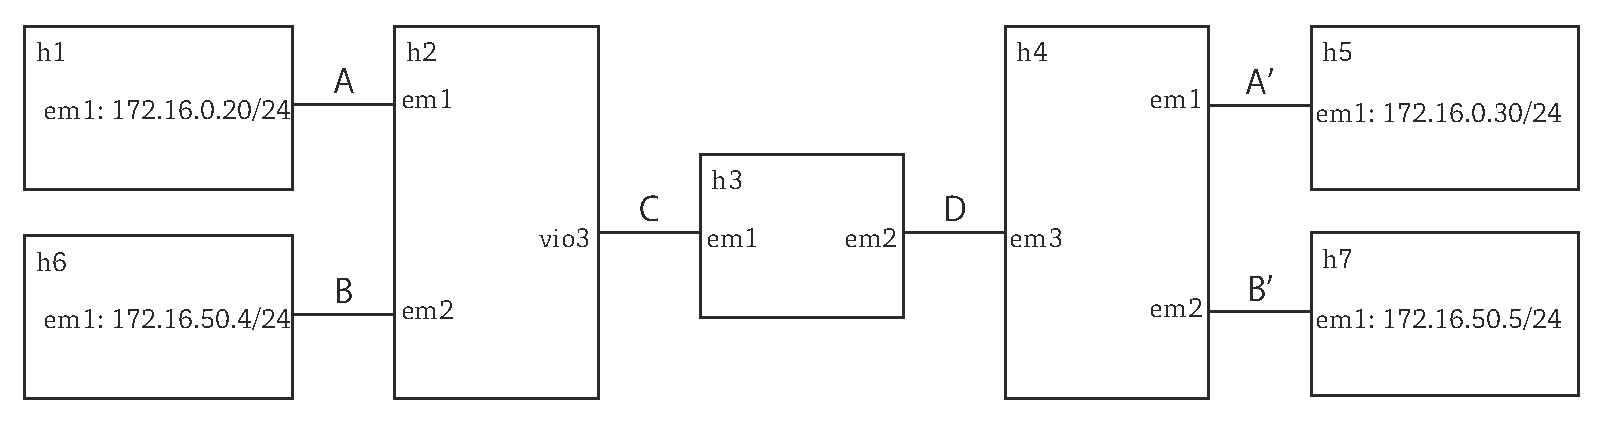
\includegraphics[width=10cm,pagebox=artbox]{figs/quiz05.pdf}
    \caption{問題5:ブリッジ実験のトポロジ図} \label{fig:quiz05}
\end{figure}

図~\ref{fig:quiz05}のネットワークがあるとする。
このとき、ノードh2でブリッジ設定、ノードh1とh3を互いに通信できるようにせよ。
ヒント:ブリッジの設定はifconfigコマンドで行える。

\subsection{問題7:VLAN}

\begin{figure}
    \centering
    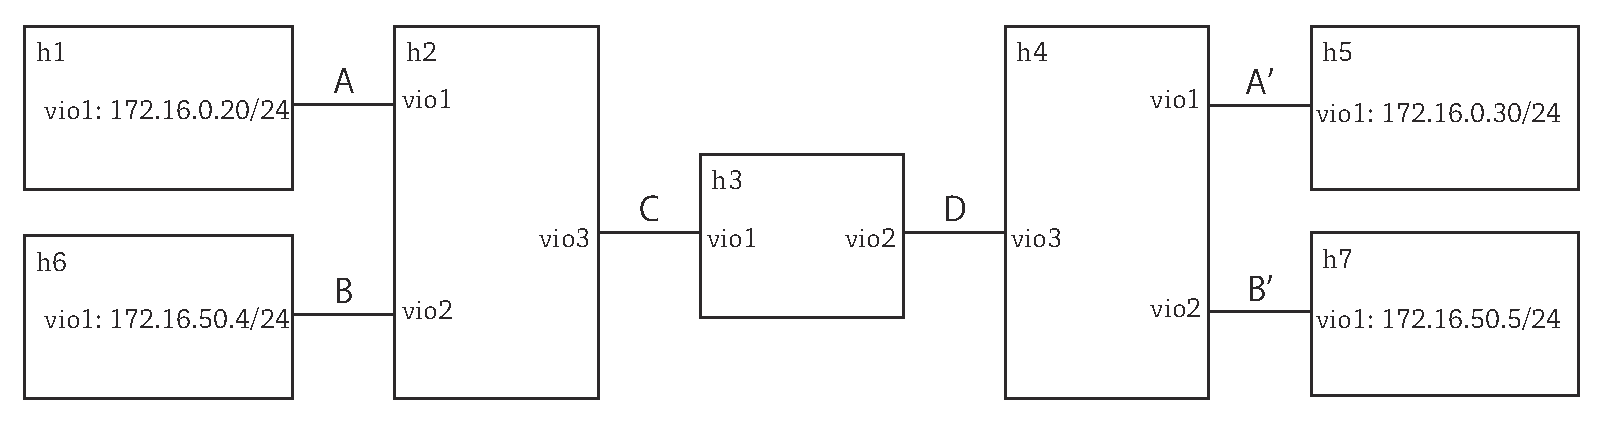
\includegraphics[width=15cm,pagebox=artbox]{figs/quiz06.pdf}
    \caption{問題6:VLAN実験のトポロジ図} \label{fig:quiz06}
\end{figure}

図~\ref{fig:quiz06}のネットワークがあるとする。
このとき、リンクAとA'が同じセグメントに、また、リンクBとB'が同じセグメントとなるように、
タグVLANとブリッジの設定をノードh2、h3、h4で行え。
ヒント:タグVLANとブリッジの設定はifconfigコマンドで行える。

\subsection{問題8:NAPT}

問題3のネットワーク設定を改変し、社内ネットワークから対外ネットワークへの接続はNAPTで接続するように修正せよ。